\section{The Problem}
\label{chap:The Problem}

 \subsection{Problem Description}
 % where does the problem arise from? problem transmission has
 %keep it short, dont go into details that tjalma can disagree with in particular about the operational part.

%%%%%%%%% IMPORTANT HERE YOU ARE!!! ############
% why even talk so much about transmissions problem. Is it relevant for what you try to show in this paper? no! Do you even clearly know the details of the problem so precisely that tjalma and gerard don't disagree with it? DO THEY??!!! remove all this talk about TransMisson. Totally Unnecessary

% overview
The VRPTT can be described as follows:
there is a set of customers with a known, deterministic supply of a single good.
There is a set of transshipment locations that may be used for parking and load transfers.
All locations have opening and closing times.
To collect the customers' supply, a fleet of heterogeneous, limited-capacity vehicles stationed at the vehicle depot is available.
Some customers can not be visited with trailers because of accessibility constraints.
While goods are collected, costs should be minimized.
A lorry ends its path if it unloads at the depot or after it decouples a trailer at the depot. \\

% fleet
The fleet of vehicles consists of lorries and trailers.
Trailers can only move if pulled by a lorry.
Not all trailers and lorries are compatible with each other.
All vehicles may have different capacities, fixed costs and variable costs.
Lorries may differ in the amount of time they need to collect a certain amount of customer supply.  There is no fixed assignment between trailers and lorries.
Trailers can be shared by multiple lorries.
Any trailer can be pulled by any compatible lorry. \\

% locs
Transshipment locations can be used by lorries to transfer load to a trailer.
There are no costs associated with coupling and uncoupling a trailer except for the cost incurred by the time it takes to finish the operation.
A vehicle will start and end its route at the depot location.

% customer
Customers that can not be visited with trailers are called lorry customers. Customers that can be visited with trailers are called trailer customers. Split collections are not allowed, hence each customer's supply is collected by one lorry.
There is no customer with a supply greater than the capacity of the lorry with the least capacity.
Trailer customer locations can also be used as transshipment locations. \\


% NP-hardness

The VRP is a special case of the VRPTT, namely an instance without transshipment locations and without trailers. Since the VRP is NP-hard \cite{laporte2009fifty}, the VRPTT is also NP-hard.



\subsection{Problem Model}

% NOTE change the language of this first part. What could a solution to the question look like. What information does it need to contain?

A solution to an instance of the VRPTT should answer the following questions:
%\begin{itemize}
%\item Which lorry collects the supply of which customers and in what order?
%\item In what order does the lorry collect the supply of customers or couple and decouple trailers?
%\item From where to where is which trailer pulled by which lorry?
%\item Which lorry is coupled to which trailer during which part of its path?
%\item When and how much load to lorries transfer to trailer?
%\item At what time does everything take place?
%\end{itemize}

\begin{itemize}
\item How should the customers be divided over the lorries and in which order should the lorries visit them to collect their the customers' supply?
\item How should the lorries use the trailers?
\item How should the load be divided between the vehicles?
\item When do all the events in the plan take place?
\end{itemize}


% A usable model will be able to represent the  answers to these questions.

\subsubsection{Simple Example}

\label{sec:simple-example}

Lets explore a simple example of the VRPTT.
In Figure~\ref{fig:trivial} we can see an illustration of a VRPTT.
For the moment we ignore some aspects of the VRPTT for the sake of clarity.
The VRPTT does not allow a vehicle to leave the depot after it visits the depot.

% Furthermore, instead of asserting the factors that need to be adressed, we could show hwo they arise from the example.
% maybe even make this subsection the first subsection in this chapter. The adept methodology says to first analogy, diagram, experience. Only then give plain english and then technical.
%technical is problem formulation subsecion.
%Plain english resembles problem description section.

\begin{figure}[!ht]
  \centering
    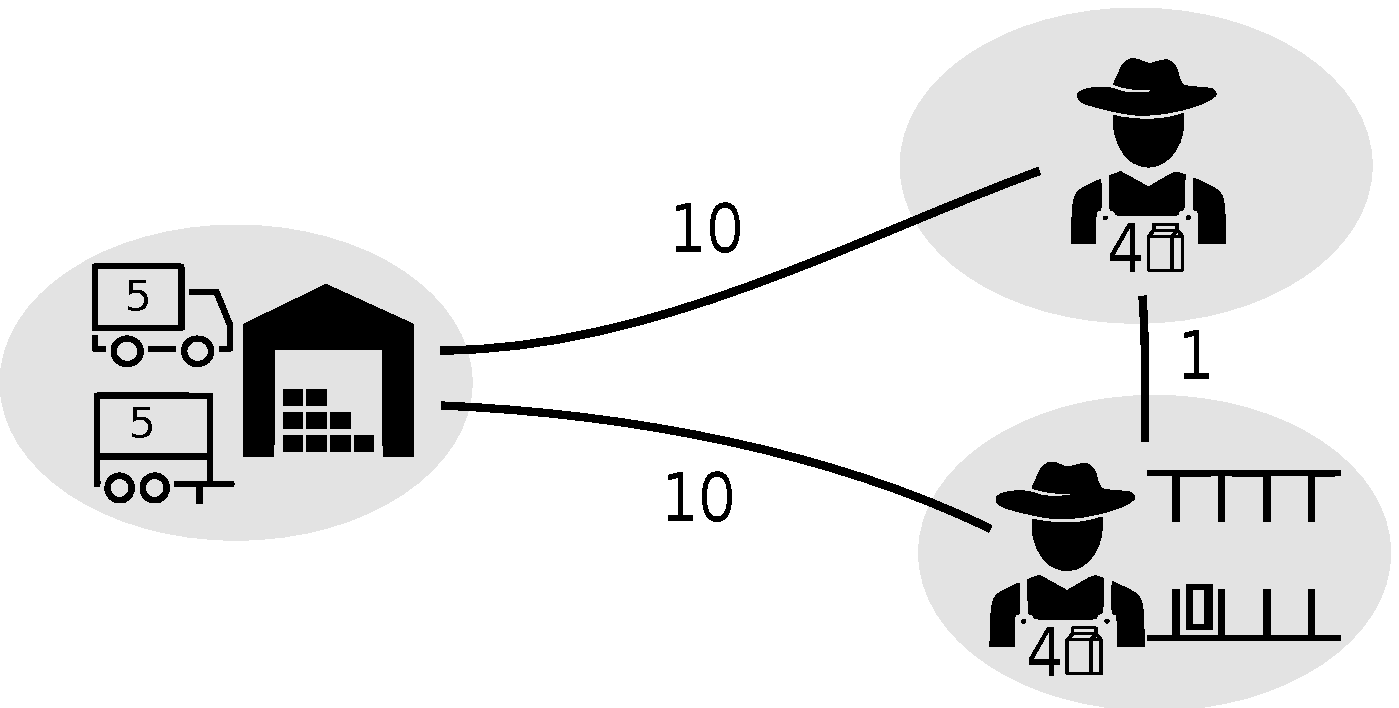
\includegraphics[width=0.8\textwidth]{img/trivial_example_withcapacity_v2.pdf}
  \caption{Illustration of an VRPTT with a trailer customer, a lorry customer and a fleet consisting of a trailer and a lorry.}
  \label{fig:trivial}
\end{figure}

% disclaimer simplification

%%%%%%%%%%%%%%%%%%%%%%
 % explain situation.
 %%%%%%%%%%%%%%%%%%%%%


% locations and fleet
The example problem contains three locations.
One of the locations is the depot.
At the depot there is a fleet consisting of a lorry and a trailer.
The other two locations are customers.
Both customers have a supply of four that needs to be collected by the vehicles and needs to be unloaded at the depot.
Both vehicles in the fleet have a capacity of five.
% distance
The customers are at a distance of one of each other and at a distance of ten to the depot of the transporter.\\

% capacity

% lorry vs trailer customer
The customer on the bottom has a parking lot, hence it has enough space to be visited with a trailer.
This customer is therefore called a trailer customer.
A location that can be visited with a trailer can be used to park a trailer and/or to transfer load from a lorry to a trailer.
Such a location is called a transshipment location.
The other customer does not have a parking lot and can therefore not be visited with a trailer, which makes it a lorry customer.\\

% model choices

% The VRPTT does not allow a vehicle to leave the depot after it visits the depot.
% The lorry can therefore not collect the supply of one customer, then unload and then service the other customer.
 % hence both customers can not  the same lorry can not be used to service both customers.
% A trailer will be immediately unloaded after a lorry decouples it at the depot and can therefore not leave after being decoupled at the depot.


% components of solution
% The transporter would like to know how he should use his fleet to collect the supply of the customers.

\subsubsection{Events}


Let us attempt to construct a plan that answers at least the first two questions that a solution to the VRPTT needs to answer.
Since vehicles are not allowed to leave the depot after visiting it, the lorry can not unload at the depot between visiting the customers.
The lorry and the trailer can not separately take care of a customer, since the trailer can not move on its own.
Since the lorry alone does not have enough capacity to collect the supply of both customers, it needs to use the capacity of the trailer.
%  transfer some of its load that it collects from to the  the capacity of the trailer in some way.
% visit the customers whilst coupled to the trailer.
% couple the trailer and p.
\\

%The trailer cannot move on its own, therefore we do not need to state its movement explicitly. It is defined by the actions of the lorry.

The lorry can not visit the lorry customer whilst coupled to the trailer.
% and the trailer can not visit the lorry customer together.
Let us say that they go to the trailer customer first. So far the plan is as follows:
\begin{enumerate}
  \item The lorry starts it path at the depot.
  \item The lorry couples the trailer.
  \item The lorry and trailer drive to the trailer customer.
\end{enumerate}
Now there are two good courses of action.
Either the lorry collects the supply of the trailer customer first or it decouples and parks the trailer first such that it can collect the supply of the lorry customer.
Let us say that it collects the supply of the trailer customers first, then the plan continues as follows:
\begin{enumerate}[resume]
  \item The lorry collects the supply of the trailer customer.
  \item The lorry transfers at least three units of the supply to the trailer such that it has at least four capacity available for the supply of the lorry customer.
  \item The lorry parks and decouples the trailer.
  \item The lorry drives to the lorry customer.
  \item The lorry collects the supply of the lorry customer.
  \item The lorry drives back to the trailer customer.
  \item The lorry couples the trailer.
  \item The lorry drives back to the depot.
  \item The lorry decouples the trailer and unloads.
  \item The lorry ends its path and unloads.

\end{enumerate}

% notice how the activities that the lorry is involved in completely defines what happens to the trailer.

This is quite a verbose description of a transport plan.
Notice that every step is either about the lorry travelling between locations or about the lorry performing an activity at a location.
% the (change of) location of the lorry (and trailer) or about an activity the lorry undertakes at a location.
This list of steps can be compressed into a list where every step consist of an activity and a location, see Table~\ref{tab:events}.
From now on this combination is called an event. The sequence of events that a lorry is involved in is its path.

\begin{table}[!h]
  \centering
  \begin{tabular}{@{}llll@{}} \toprule
  %  \multicolumn{2}{c}{Event} \\ \cmidrule(r){1-2}
    Event \# & Location & Activity & Event ID  \\ \midrule
    1 & depot & start path & A \\
    2 & depot & couple the trailer & C \\
    3 & trailer customer & collect supply & F \\
    %4 & trailer customer & transfer load & lorry and trailer \\
    4 & trailer customer & decouple the trailer & G \\
    5 & lorry customer & collect supply & E  \\
    6 & trailer customer & couple the trailer & H  \\
    7 & depot & decouple trailer & D  \\
    8 & depot & end path  &  B \\     \bottomrule
  \end{tabular}
  \caption{The events in the plan.}
  \label{tab:events}
\end{table}

Notice that the load transfer from the lorry to the vehicle is not treated as a separate event.
This is because we allow the load to be transfered from the lorry to the trailer at any event as long as they are coupled.
In this case the transfer happens in either event three or four and the amount that is transfered lies between three and four such that the lorry has enough capacity to collect the supply of the lorry customer.\\
% Later in more detail how the transfer of load is represented from the lorry to the trailer.
 % on that we can determine how to divide load between lorry and trailer without using such an event in our model.

Notice also that by choosing to park a trailer, two events are created. A trailer needs to start and end its path at the depot, hence if it is decoupled at some transshipment location it needs to be coupled again there as well. \\






\begin{figure}[!h]
  \centering
    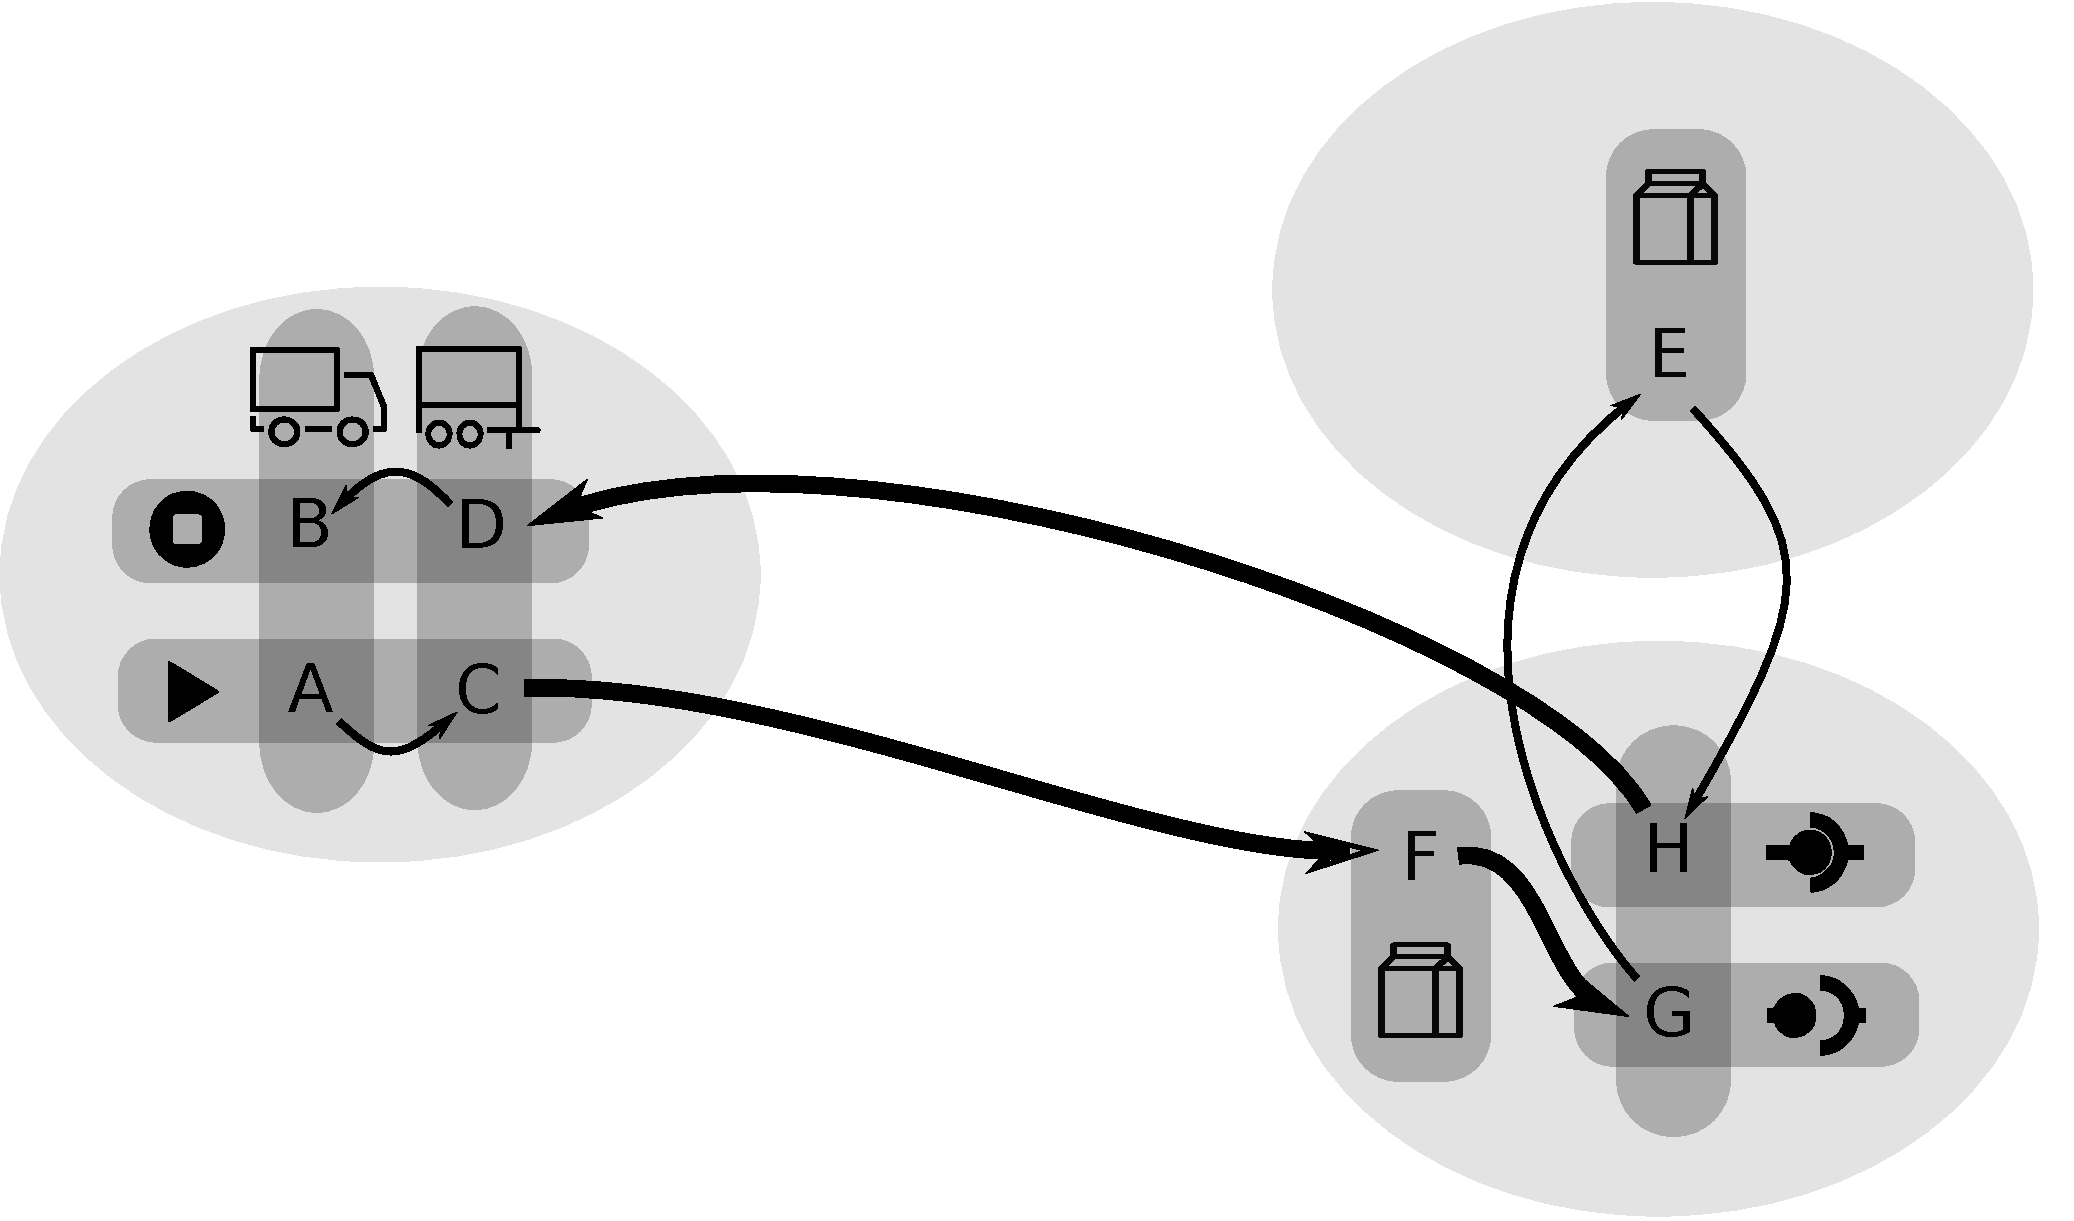
\includegraphics[width=0.8\textwidth]{img/trivial_vertices_v2.pdf}
  \caption{An illustration of the lorry's path. Every event is indicated with the event ID supplied in Table~\ref{tab:events}. The activity of the event is illustrated with a symbol. The position indicates the location of the event. The fat lines indicate where the lorry is coupled to the trailer. The thin lines indicate where the lorry is not coupled to the trailer.}
  \label{fig:vertices}
\end{figure}



If we look at Figure~\ref{fig:vertices} we can see all the events in our plan and the path of the lorry.
From the path of the lorry we can infer the path of the trailer, namely it starts at $C$, then we follow the fat line to $ F $ and $ G$. Transshipment events come in pairs, a couple event and a decouple event. A trailer decoupled at $G$ can be coupled again at $H$.
 % This is a movement through time, not space.
 From $H$ we follow the fat line back to $D$. \\

Notice that each event in the plan is unique, in that it occurs only once in the path of the lorry.
% by constructing the plan in terms of events every element of the plan only occurs in the path of the lorry once.
Furthermore, notice how we can answer the first two questions that a solution to the VRPTT needs to answer by looking at the path of the lorry.


\subsubsection{Load Division}

% The capacity of the vehicles is limited.
% Given the path of the vehicles, how should we use their capacity such that the supply of the customers can be collected and unloaded at the depot whilst not overloading the vehicles?\\

The third question that needs to be answered is about how, given the events of a plan, the customer supply ends up at the depot.
 % by flowing through the vehicles.
% flows from the customers through the vehicles, to the depot.
The vehicles have a limited capacity, so they need to coordinate how load is divided between them.
This is done by determining at which event of the plan a load transfer from a lorry to a trailer needs to take place and the amount that needs to be transfered.
% the amount of load that needs to be transfered from a lorry to a trailer, and the event at which this needs to happen.
\\




%  load flows from customers to the depot.
% This is the third question a solution to the VRPTT needs to answer.
% Furthermore, is it even possible to collect all the supply without overloading the vehicles given the paths of the vehicles?

% To determine this we need to track the flow of the load from the customers to the depot.


\begin{figure}[!h]
  \centering
    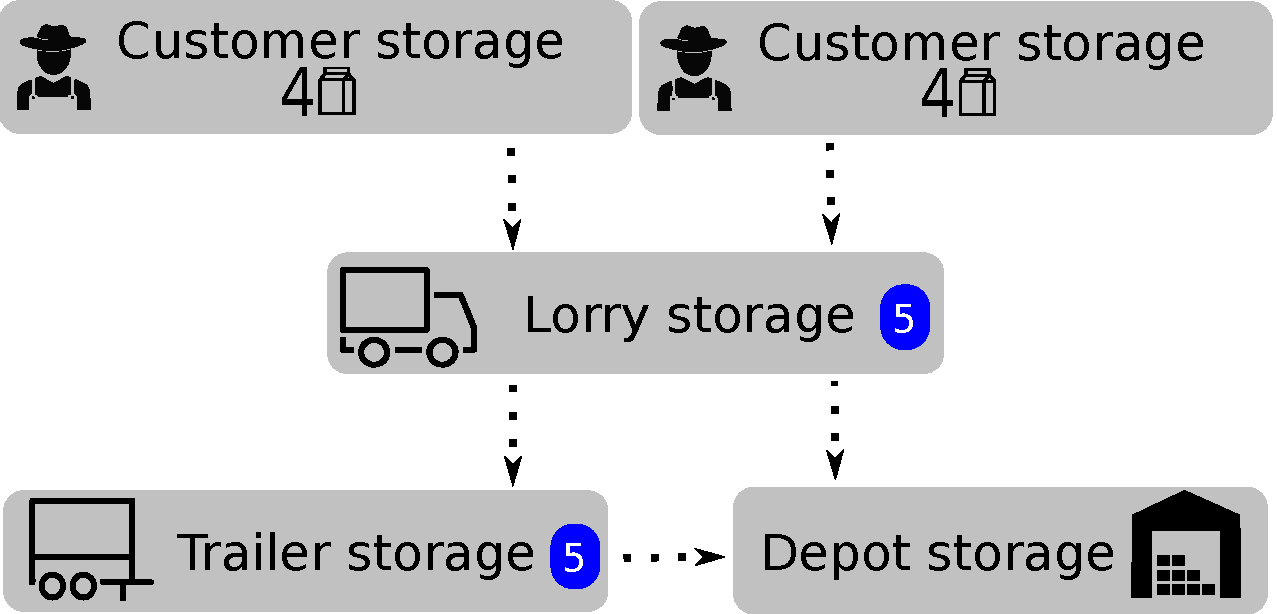
\includegraphics[width=0.8\textwidth]{img/trivial_flow_simplified_v2.pdf}
  \caption{An illustration representing how load can flow from the customers to the depot. The amount of supply of the customers is indicated with the milk icon and the capacity of the vehicles is indicated in blue. }
  \label{fig:flow_simplified}
\end{figure}

The customers' supply flow from customers to the depot as presented in Figure~\ref{fig:flow_simplified}.
The only sources of supply are the customers, both with a supply of four.
The only sink for the load is the depot.
The supply can reach the depot by flowing from a customer to the lorry and then to the depot.
Alternatively, supply can flow from a customer to the lorry, then to the trailer, then to the depot.
Before the vehicles can be finished with collecting all eight units of customer supply, at least three units of supply must have flown to the trailer, since the lorry can only hold five units of supply at any one time.
No more than five units of supply can have flown to the trailer in total, since it can only hold five units.
Notice how the lorry can decrease its amount of load before unloading at the depot, but that the trailer can not.  \\

% Before all of the supply of the  supply of the second customer can be collected at least some of the load has to flow to the trailer.  since the sum of the customer supplies (eight) is greater than amount of load that the lorry can hold at once (five).

% The question is: when and how much of the load is transfered to the trailer such that the vehicles ares not overloaded?
% Figure~\ref{fig:flow_simplified} does not offer enough detail to answer this question.
% See Figure~\ref{fig:flow} for greater detail.



\begin{figure}[!h]
  \centering
    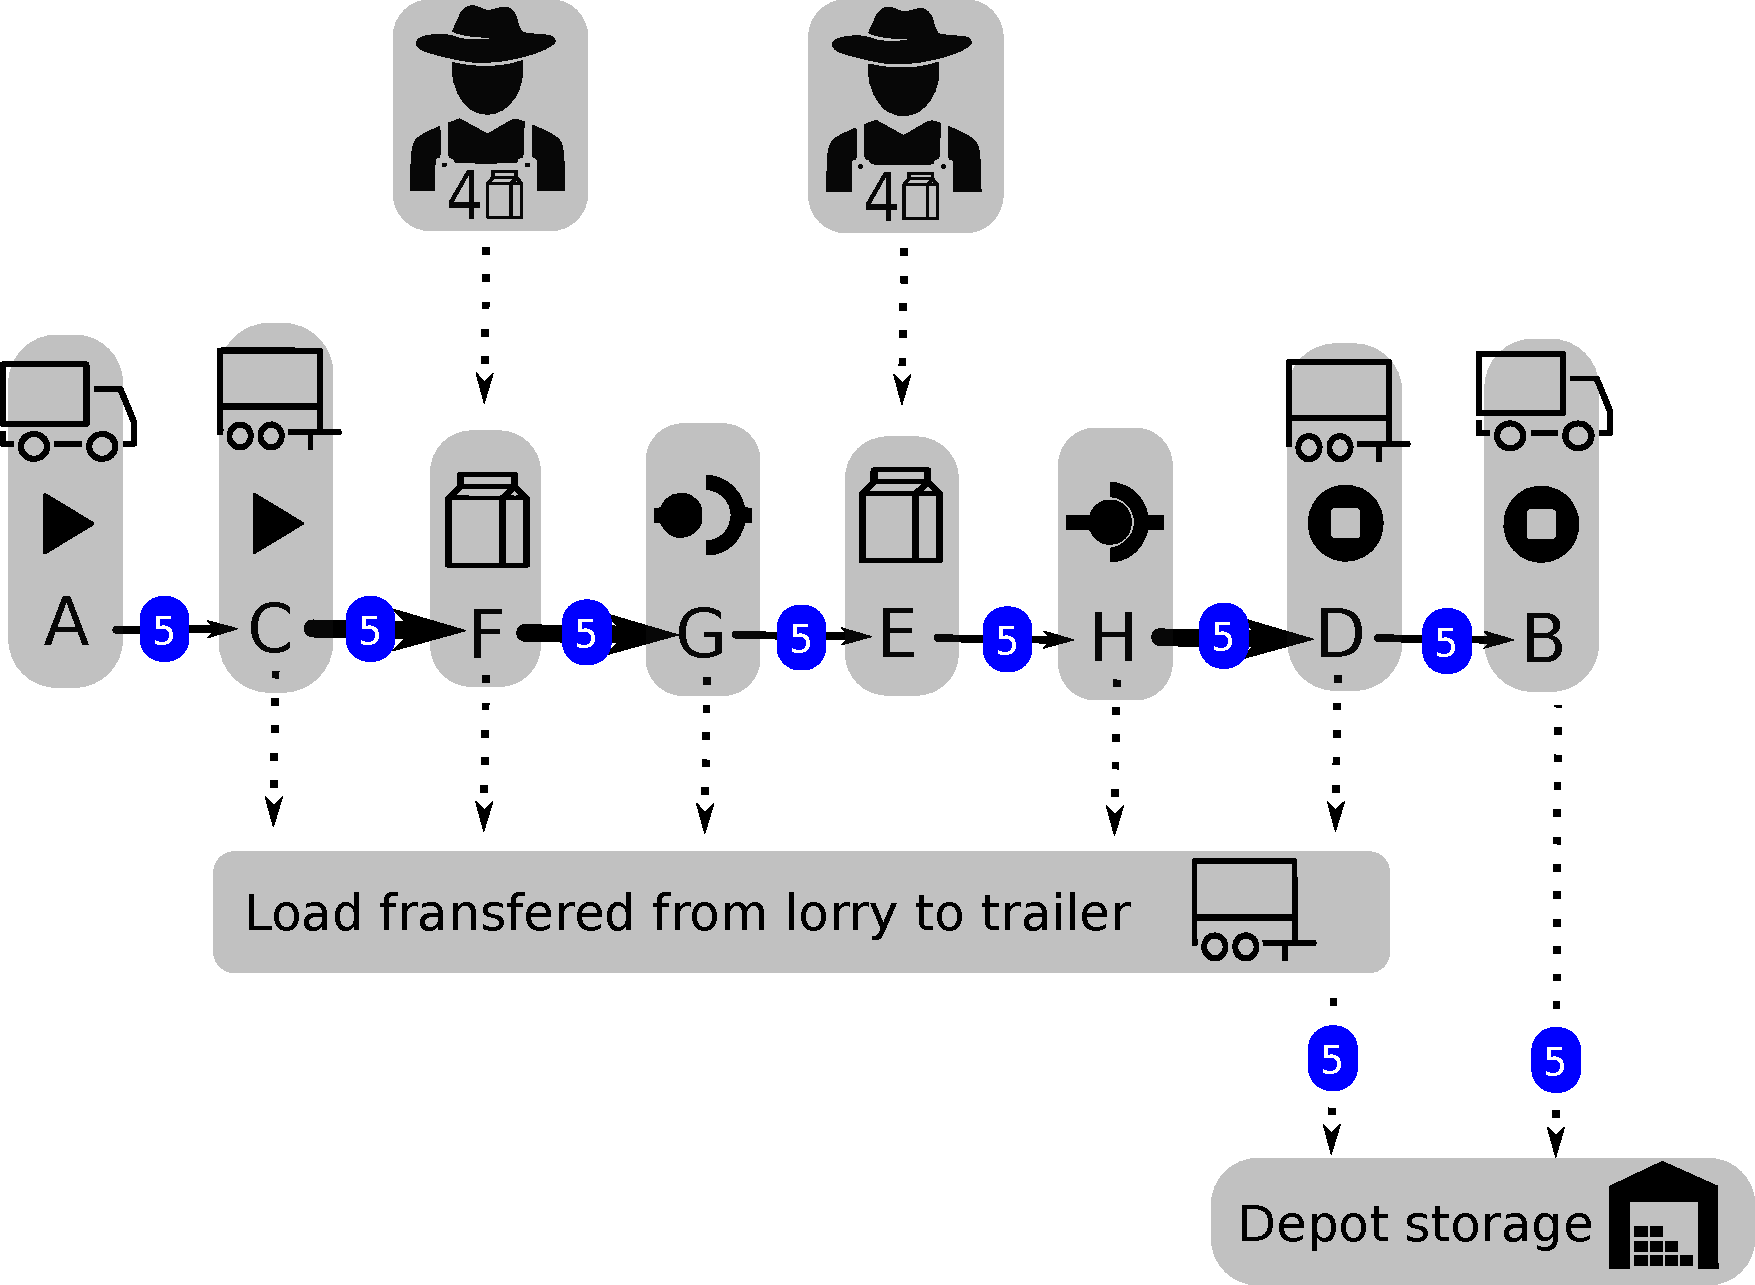
\includegraphics[width=0.8\textwidth]{img/trivial_flow_v2.pdf}
  \caption{The load division problem. Dashed arrows represent the ways that load can flow. If flow restrictions exist, they are indicated in blue.
 Arrows indicate how load can flow from event to event as cargo inside the lorry.
 Fat arrows indicate when the lorry is coupled to the trailer.}
  % The amount of customer supply is indicated with the milk icon.}
  \label{fig:flow}
\end{figure}

To not only determine the amount of supply that needs to be transfered, but also the event at which the transfer needs to take place, we need to consider the flow of supply per event. The ways supply can flow at each event is illustrated in Figure~\ref{fig:flow}.
Every time the lorry is at an event, it can choose to transfer load to the trailer, if they are coupled.
% In Figure~\ref{fig:flow} we see all the events in the path of the lorry.
% At the events where the lorry is coupled to the trailer, load can flow from the lorry to the trailer.
At the supply collection events, $F$ and $E$,  load can flow from a customer to the lorry.
When the lorry ends its path at the depot, event $B$, load can flow from the lorry to the depot.
The only time load can flow out of the trailer is when it decouples at the depot, event $D$ .
The maximum amount of load that can flow from a vehicle to the depot is equal to its capacity, which is five for both vehicles.
We can ensure that the trailer is never overloaded during its path if we constrain the amount of flow from the trailer to the depot to the trailer's capacity, since that is the only time that load can flow out of the trailer.
Load can flow into and out of the lorry at multiple events, therefore we have to restrict the flow between events to the lorry's capacity such that during its path it never carries more load than its capacity.
\\



%Lets look at Figure~\ref{fig:vertices} and imagine how the supply of the customers can flow from the customers, %through the lorry and possibly through trailer, to the depot. Keep in mind that the fat line indicates where the %railer and lorry are coupled, and that the lorry can transfer load to the trailer at any event where they are %coupled. This situation is summarized in Figure~\ref{fig:flow}.




% TODO To check this in a more systematic way instead of eyeballing, we turn this problem into a weighted digraph using thefollow trick and use a max flow algorithm.


%
% We can eyeball that if the supply of the customer that is visited first, flows from the customer to the lorry and then straigth into the trailer and the supply of the second visited customers is just kept inside the lorry, then all the supply of each customer can be collected without overloading any vehicle.
%
% But instead of eyeballing the solution like this, we can also find a solution by solving the a max flow problem.

This problem of dividing load between vehicles can be abstracted to a maximum flow problem, see  Figure~\ref{fig:flow_abstract}.
The maximum flow problem asks how much load can transfer from a source to a sink.
The vertices of the maximum flow problem consist of the events of the plan, a special vertex $P$ for the trailer to show the flow of load from the lorry to the trailer,
one sink $sink$ and one source $source$.
% A max flow problem has vertices, capacitated edges and one source and one sink.
We already have one sink, which is the depot.
However, we have two sources of supply, which we replace with one source.
The source has an edge to a customer's supply collection event with a capacity equal to the customers amount of supply, such that the maximum amount of supply that can be collected at the customer's is maintained.
We have already determined where and how much load can flow, which is reflected in the rest of edges and the edge capacities. \\
% The edges reflect how supply can flow between the vertices with capacities that reflect how much load can flow over the eg.
% To represent load flowing to the trailer we have added the vertex


% In our situation we have two sources.
% We can change this by adding a supersource $S$ connected to the customers $S'$ and $S''$  and by restricting the flow from the supersource to the customers to the amount of their supply.



\begin{figure}[!h]
  \centering
    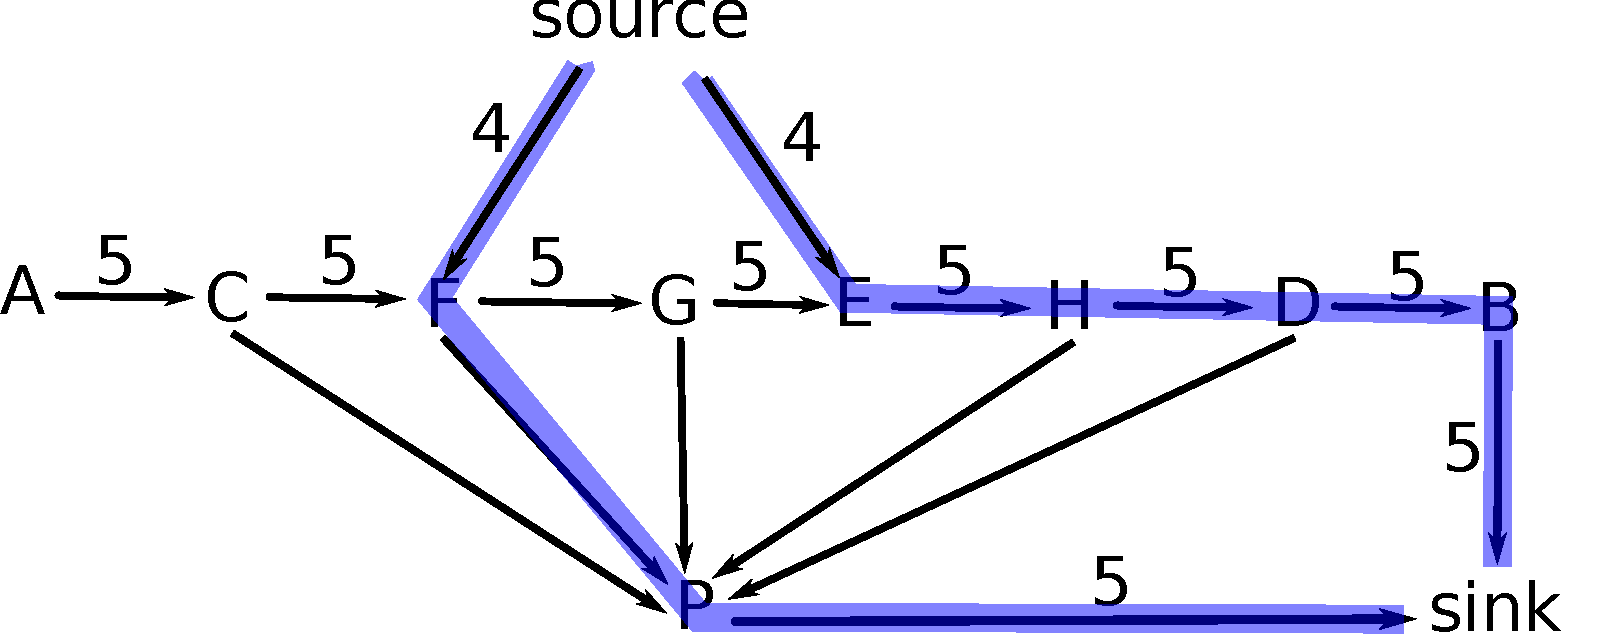
\includegraphics[width=0.8\textwidth]{img/trivial_flow_abstract_BlueFlow_v2.pdf}
  \caption{A directed graph representing the load division problem. If an edge has a limited capacity, the capacity is shown.}
  \label{fig:flow_abstract}
\end{figure}

% In Figure~\ref{fig:flow_abstract} we illustrate the situation as a graph with a few changes.
%
% Load that is transfered to the trailer, flows to vertex $P$. This vertex is sort of a pool which gathers all the load that gets transfered from the lorry to the trailer.


% This would result in the load table of Table \ref{tab:loadtable}. The load table describes how much load a lorry has when leaving an event. \\

%
% \begin{table}[!h]
%   \centering
%   \begin{tabular}{@{}lllll@{}} \toprule
%   %  \multicolumn{2}{c}{Event} \\ \cmidrule(r){1-2}
%     Event \# & Location & Activity & Event ID & Load \\ \midrule
%     1 & depot & start path & A & 0 \\
%     2 & depot & couple the trailer & C & 0 \\
%     3 & trailer customer & collect supply & F & 0 \\
%     %4 & trailer customer & transfer load & lorry and trailer \\
%     4 & trailer customer & decouple the trailer & G & 0 \\
%     5 & lorry customer & collect supply & E & 4 \\
%     6 & trailer customer & couple the trailer & H & 4 \\
%     7 & depot & decouple trailer & D & 4 \\
%     8 & depot & end path  &  B & 4\\     \bottomrule
%   \end{tabular}
%   \caption{The load table corresponding to the flow in Figure \ref{fig:flow_abstract}.}
%   \label{tab:loadtable}
% \end{table}
%\begin{figure}[!h]
%  \centering
%    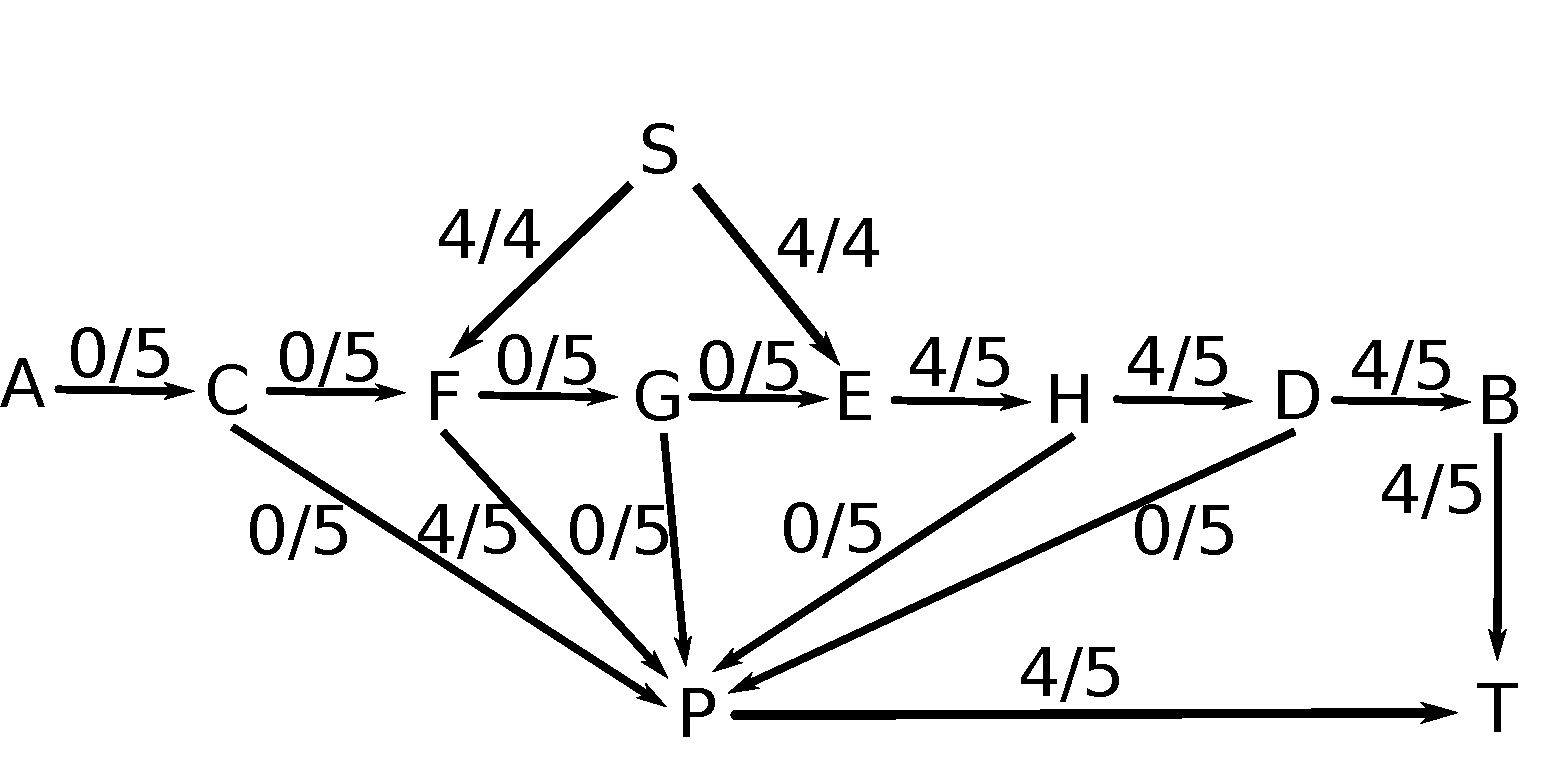
\includegraphics[width=0.8\textwidth]{img/trivial_flow_solution.pdf}
%  \caption{A directed graph with the capacity on the edges and a flow that is a solution to the max flow problem from source $S$ to sink $T$.}
%  \label{fig:flow_solution}
%\end{figure}


A possible solution to this max flow problem is a flow of size four on path $\{S,F,P,T\}$ and a flow of size four on path $\{S,E,H,D,B,T\}$. This is the solution illustrated in Figure~\ref{fig:flow_abstract}.
The third question a solution to the VRPTT needs to answer can thus be solved by solving a maximum flow problem.
%interpret results
% In the suggested solution only at event $F$ which corresponds to collecting load at the trailer customer, a load of size four was transfered from the lorry to the trailer.
% possible
\\

If the maximum flow is smaller than the sum of the customers' supply, we know that given the current event plan no way of dividing the load between the vehicles exists, that would allow us to collect all the customers' supply.
Not creating a separate event for load transfers has enabled us to infer this.
% Being able to infer this is what not creating a separate event for load transfers has done for us.

% answer fourth question
% By looking at the paths of the lorries it can be seen for each event whether and which trailer the lorry was pulling . Given that we know for each event whether and how much load was collected there by the lorry, we can also answer whether and how much load was transfered to the trailer by looking at the load of the lorry at each event.

%\todo{in this case it is easy enough to eyeball how load needs to be balanced such that the lorries have enough capacity to pickup the supply of the customers. And even that it is possible. But how do we formally check this? }





% separate decouple and couple because if I want to assign a time or I want to say that one thing has to happen before something else, I should have 2 vertices. Otherwise it also has 2 successors.



% you don't need separate description of what the trailer does. Everything is described of the lorry taking actions.



%Which components does a transport plan consist of?  In this example the transport plan needs to describe the movements of the lorry and the trailer.



% driving cost
%The cost per distance unit of the lorry and the trailer is one and $0.1$ respectively.


% time parameters
%Lets say that the maximum speed of the vehicles is 1 distance unit per time unit and that it takes 2 time unit to load 5 milk units
%The objective function that we need to minimize is the sum of the HERE YOU ARE!

% what argument can I give for the structure of vertices without invoking time.
% - I could say that to make a solution I need to describe the movement of the vehicles. I can do this even without capacity.


% all information till here is visible in picture. Perhaps first deal with this case and only then introduce the factor time for which the parameters are given below.
% Lets recap: we can answer the first three questions a plan needs to adress by looking at the path of the lorry and by tracking its load at each events on its path.




\subsubsection{Timing.
At what time should each event take place, such that there is enough time to perform each event, travel between events, such that the time windows are notS violated and the least amount of time is spent just waiting till a location opens. ??Added preference; we would like to do everything as early as possible?? if start and end time are fixed, we would liike to do everything as early as possible (because of slack and because that is just how I defined that it works. Lorry starts as soon as arrives or as sson as openss. does not wait at vertex. also becasue there is no slack than anymore) }

% In the previous section we talked about the flow of load, now we will talk about the flow of time.
% The flow of time can best be described using a time table that describes the time at which a lorry arrives at an event.
% An event represent a lorry that changes locations or a lorry performing an activity at a location.

% TODO The time at which a lorry arrives at a location can thus be interpreted as the time at which the lorry is ready to start the event.

% The time table describes the starting time of each event.
% A time table indicates at what time a lorry needs to start on its path and
% the duration of the lorry's path can be .
% Another use of a time table is that we can verify whether the paths of the lorries satisfy the time constraints of the locations.

The fourth question that needs to be answered is about at what time the events of a plan  take place such that costs are minimized and the locations' time windows are not violated. In this example the amount of time that the fleet uses is used as a proxy for costs.
\\

To illustrate the problem we extend the example of Section \ref{sec:simple-example} with time windows, travel times, event durations and a planning horizon.
The planning horizon in this example is the interval [0,22] hours.
The rest of the time related information is provided in Figure ~\ref{fig:graph_time}. \\

% , the customer supply ends up at

\begin{figure}[!h]
  \centering
    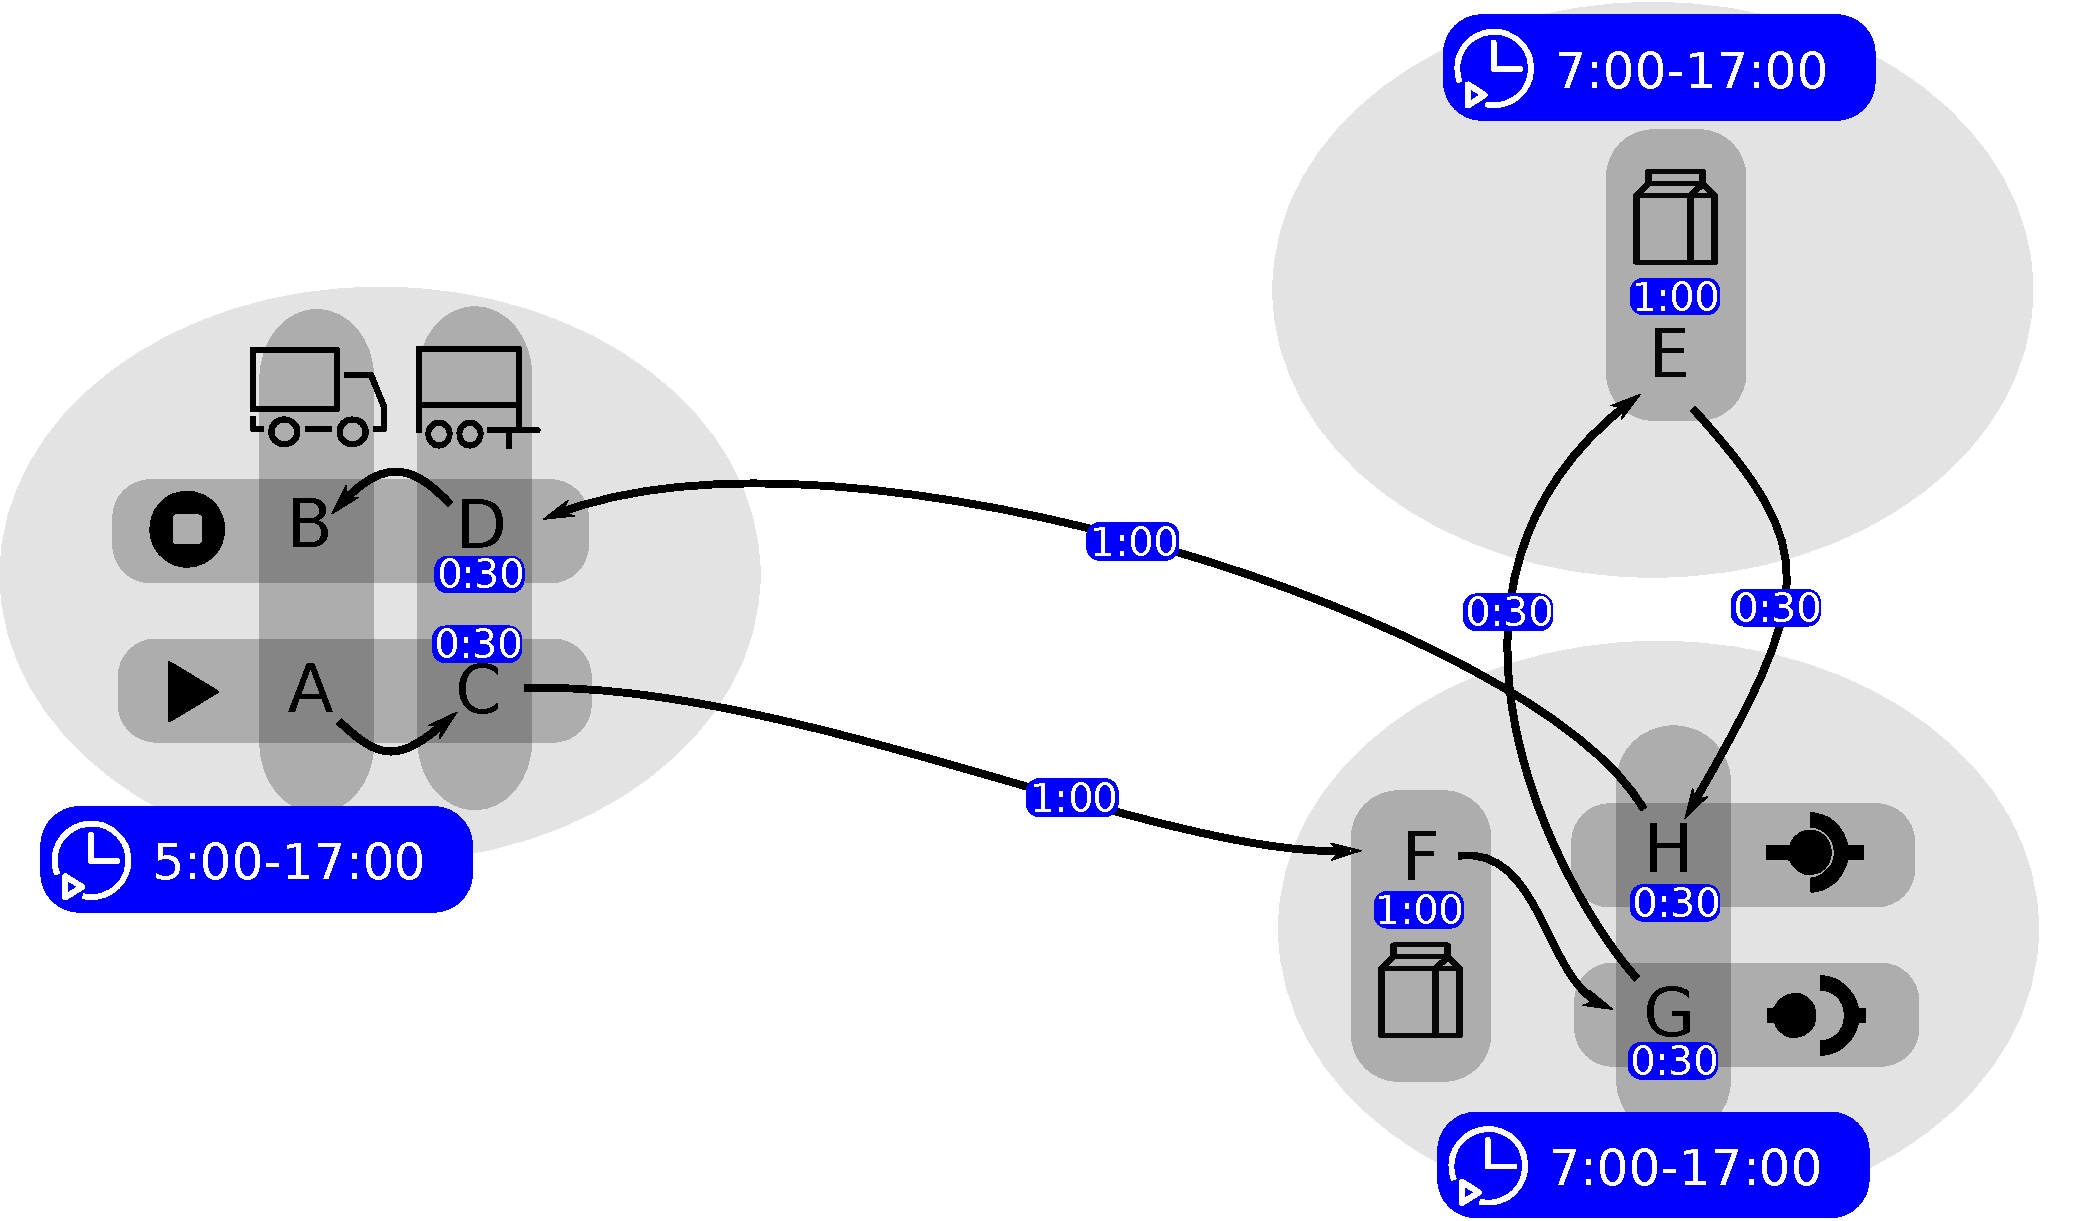
\includegraphics[width=0.99\textwidth]{img/example_with_time_v2.pdf}
  \caption{An illustration of the lorry's path with time information illustrated in blue in hours. Each location has a time window that holds for all events at that location.
 If no time information is provided the travel duration or event duration is zero.
 As Figure ~\ref{fig:graph_time} illustrates, some events don't take up any time and going from event to event on the same location does not take up any time.
  %  If an event has a nonzero duration or if there is nonzero travel time between events , the time is indicated in blue.
   }
  \label{fig:graph_time}
\end{figure}


This problem can be turned into a longest path problem.
In Figure ~\ref{fig:graph_time} it can be seen that
An abstraction of the problem  in the previous section can be made.
% Both customers have a supply of size four.
% Say the lorry has a loading speed of four per hour.
% Then the duration of collecting the supply at a customer, indicated in Figure ~\ref{fig:graph_time} with a question mark, is exactly an hour.

Enough information is provided to determine the earliest time at which the events in the lorry's path can take place.
Preferably this

This is done by constructing a precedence graph.
With this information it can the

To show how we can calculate a timetable from the path of the lorry we represent the situation again as a graph.
Every vertex represents an event in Figure ~\ref{fig:graph_time}.
We remove the weight on the vertices by duplicating every vertex.
Every event now corresponds to a start vertex and an end vertex.
The duration of the event will now be represented by the weight of the edge between the start and end vertex of the event. We can see this illustrated in ~\ref{fig:duplication}



% TODO The question marks at the customers' indicate that the duration of collecting the supply is dependent on the loading speed of the vehicle.

% TODO create easy example of pert diagram. use same symbols s to t. Say we have several jobs to do that dpened on eachother in the following way.

% TODO clearly define which question you answer. Deadline missing boolean? schedulng? Do i use edges from events to sink for end time window???
Furthermore,

\begin{figure}[!h]
  \centering
    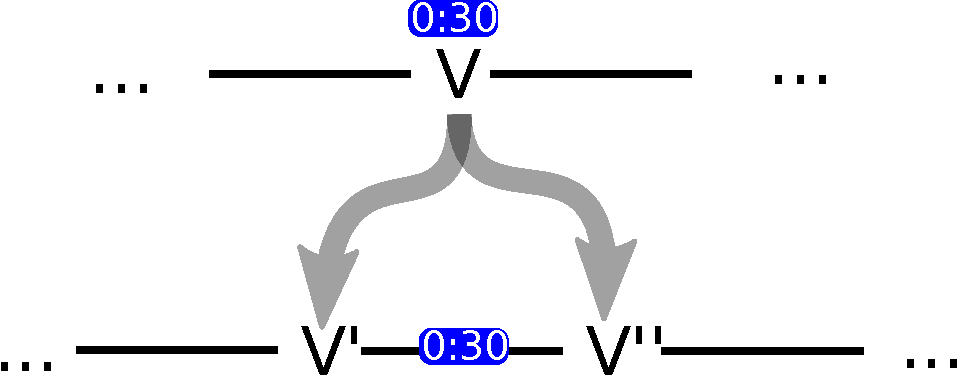
\includegraphics[width=0.8\textwidth]{img/pert.pdf}
  \caption{FIXME}
  \label{fig:duplication}
\end{figure}

We can take time relative to the depot start time since no action can be taken before the depots opens up.
A fixed amount of time is planned for the load transfer independent of the amount of load that is actually transfered.
This is a sensible assumption when the setup cost is the determining factor
for the duration of a load transfer.

% TODO explain that where the load is tranfered is of no consequence for the time table. It is either at a customer where it can  be loaded straight to the trailer, or at a TL loc. and the time it will take is always less than the time that we have reserved for TL



% TODO perhaps I should also make a small example that shows a dynamic time window with 2 lorries. Use this opportunity as well to explain that there can be no cycle.
\begin{figure}[!h]
  \centering
    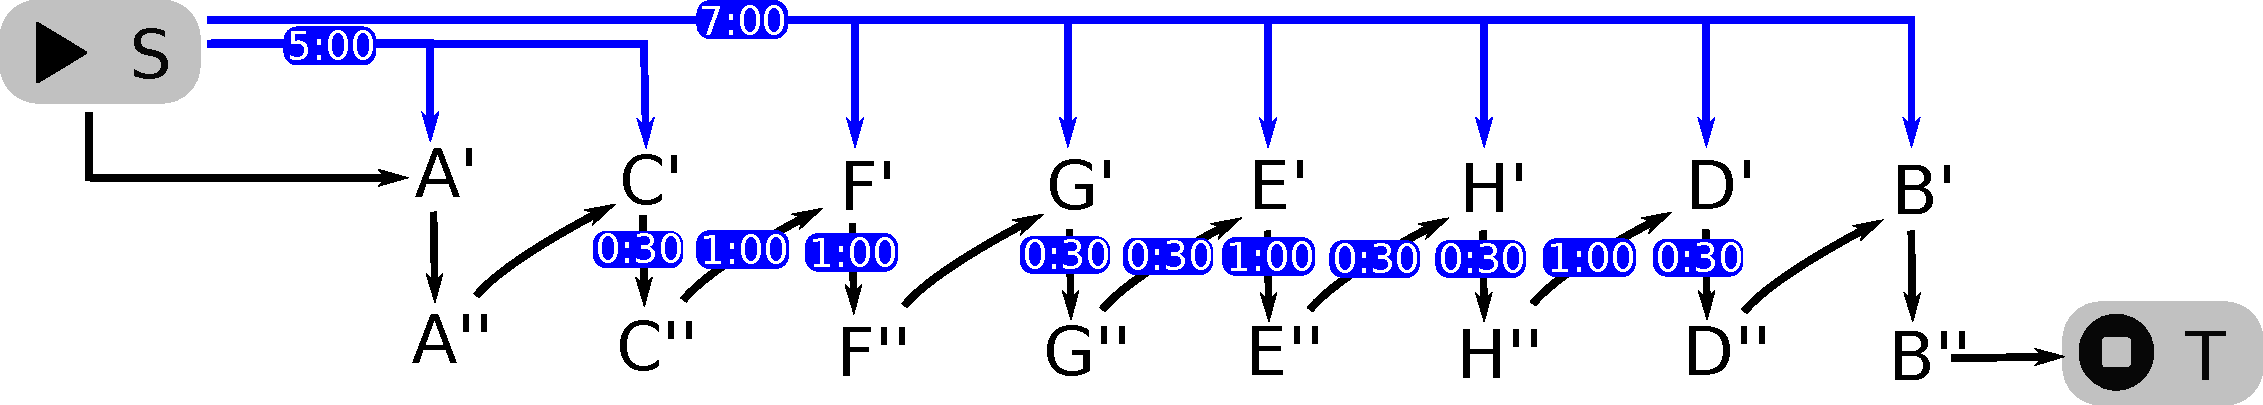
\includegraphics[width=0.8\textwidth]{img/example_time_duplicates_nozero.pdf}
  \caption{FIXME}
  \label{fig:longest_path}
\end{figure}



\subsubsection{Multiple Trips}
% , the model without this constraint  will be named after the main consequence of removing this constraint; the vehicle routing problem with transfers, transshipments and multiple unloads (VRPTTMU) }%:
In the VRPTT a trailer can only be coupled by a lorry at the depot if this is the first thing a lorry does after starting its path.
Furthermore, after the lorry decouples a trailer at the depot is has to end its path.
The VRPTT can be extended in a useful way by removing these limitations. \\

% , if the lorry visit
% An useful extension  to the VRPTT can be made by allowing a lorry to visit a trailer couple vertex at the depot

% unload at the depot or decouples a trailer at the depot witout ending its path.
% A lorry can then perform multiple trips which may lead to less costs.
% This extended version of the VRPTT is from now on referred to as the vehicle routing problem with transshipment, trailers and multiple unloads (VRPTTMU). \\
%
% The following constraint is added such that the model is similar to the model in ~\cite{drexl2014bandc}, such that findings from that paper can be used for benchmarking purposes.
% The result of this constraint is that a lorry can couple (decouple) a trailer at the depot if and only if it is the first (last) thing it does on its path,
%
% \begin{align}
%   \label{con:extra}
%   x^{k}_{i,j} = \ &  0, \\
%   \quad (i,j) \in \  & \{  (u,v) : u \in V \setminus  M^+  , \ v \in N^+  \} \cup \notag \\
%    & \{  (u,v) : u \in N^- , \ v  \in V \setminus   M^-   \} ,\notag \\
%   \ k \in \ & \mathcal{F}^{\rm lorry} . \notag
% \end{align}
% % -------------------

% Use a semi-colon between two main clauses if they are not separated by and, or etc.
%
% Example: The rain stopped; the sun came out again.

If lorries are not limited anymore to only coupling (decoupling) trailers at the depot at the beginning (ending) of their path, the following situation may occur:
% From now on we will refer to the problem that emerges when (\ref{con:extra}) is removed as the vehicle routing problem with trailers and transshipments and multiple unloads (VRPTTMU).
a lorry is full after collecting customer supply;
 the lorry couples a trailer at the depot and transfers load to it; the lorry decouples the trailer again, without the trailer even having left the depot; the lorry goes to the next customer to collect its supply.
The trailer functions in such a case as an unloading dock.
This de facto removes the restriction that a lorry can only unload once at the depot.
Therefore this model will be named the vehicle routing problem with trailers, transshipments and multiple unloads (VRPTTMU). \\

% When  lorries are not limited anymore to only coupling (decoupling) trailers at the depot at the beginning (ending) of their path, which reflects most real-life situations.
% % From now on we will refer to the problem that emerges when (\ref{con:extra}) is removed as the vehicle routing problem with trailers and transshipments and multiple unloads (VRPTTMU).
% This may result in a strange situation where a lorry couples a trailer at the depot, transfers load to it and immediately decouples the trailer again, without the trailer even having left the depot.
% The trailer functions in such a case  as an unloading dock.
% This de facto removes the restriction that a lorry can only unload once at the depot.  \\

% This situation has some problems. Trailers will still incur their fixed costs even though de facto no trailer is used. Furthermore, this usage of trailers reduces the amount of available trailers that can be used as actual trailers. To resolve this issue, synthetic trailers are added to the model without fixed costs, with infinite distance costs per distance unit and an infinite capacity to function as unloading docks for the lorries.
% These trailers will never be used as actual trailer due to their distance costs.
% % Therefore the costs incurred by a lorry that uses such a synthetic trailer as unloading dock are the time that it takes to couple and decouple at the depot.
% \\
%
% In the VRPTT these synthetic trailers don't have an impact on the best found solutions.
% If a lorry would couple such a synthetic trailer, it will have to be the first event on its path after starting its path.
% After coupling the trailer the lorry will either move away from the depot and incur infinite distance costs or go to the synthetic trailer's decouple vertex after which the lorry will have to end its path without having contributed at all to the collection of customer supply.
% Using such a synthetic trailer as an unload dock does incur the costs
% The only cost using such a synthetic trailer still incurs is the impact that the added time time costs of coupling and decoupling the trailer at the depot. In this paper this is assumed a close enough approximation to the real-life situation. Furthermore, since this is a new model feature, any choice of parameter value is arbitrary.   \\

% On the other hand,
% any choice I make for the time costs of unloading at the depot is doomed to be quite arbitrary and to obscure the effect that this new feature has on the solutions to the VRPTT. Therefore, we accept no costs for unloading as a reasonable choice.\\
%
% Then again, if I use a correction in the costs function I can just introduce one new parameter that indicates the cost. I can argue about what it shoud be in the results section. \\
%
%
%
% To keep things simple, I do not introduce a new set of vertices that belong to special unloading trailer that have 0 duration. The time that it takes to unload at the depot is now modeled to be equal to the time that it takes to couple and decouple a trailer at the depot, which seems seems reasonable.
% \\





% TODO Drexl writes "for each arc ... is the traversal time, which is assumed to be the same for all
% vehicle classes ". For costs of Drexl's no-time VRPTT it does not matter. For time TTRP i do not know whether he uses the same speed for all vehicles. Probably he uses slowest speed such that all solutions are feasible.
% On the other hand I use the vehicles speed. Not some approx.


% \subsubsection{Multiple Unloads}
% If you want to somewhat simulate the case where it is allowed for a lorry to unload multiple times, then change the objective function somewhat such that trailers that only go from N+ to N- don't cost anything. These are now defacto extra unload docks.
%
%



% towards solution
%
% \subsection{Problem Formulation}
%
%
%
%
% % +"A VRPTT instance $(\mathcal N, \mathcal A, \mathcal V, \mathcal R)$ consists of a set $\mathcal N = \{1,\ldots, N\}$ of vertices, a set $\mathcal A = \{1,\ldots, A\}$ of arcs,  a set $\mathcal V = \{1,\ldots, V\}$ of vehicles, and a set $\mathcal R = \{1,\ldots, R\}$ of requests. Let $\mathcal L = \{ {\rm depot}, {\rm lorry customer}, {\rm trailer customer}, {\rm TL} \}$ be a set of location types. Each vertex $n \in \mathcal N$ has a location type $\ell_n \in \mathcal L$. Etc."
%
%  %Note that each vertex is automatically given a number, and that you can easily define sets of certain types of vertices as $\mathcal N^\ell = \{n \in \mathcal N: \ell_n = \ell\}$ for $\ell \in \mathcal L$.
%
% A VRPTT instance $(\mathcal L, \mathcal D, \mathcal F)$ consists of
% a set $\mathcal L := \{1,\ldots, \text{n}^{\rm loc}\}$ of locations,
% %a distance matrix $ \mathcal D = \{1,\ldots, (n^{\rm loc})^2\}  $ of pairwise distances between the locations,
% a distance matrix is a mapping  $ \mathcal D := \mathcal L \times  \mathcal L \rightarrow  \mathbb{R}$ of pairwise distances between the locations and
% a set $\mathcal F = \{1,\ldots, \text{n}^{\rm veh}\}$ of vehicles.
% \\
%
% % location
% Let $\mathcal L^{\rm types} = \{ {\rm \text{depot}}, {\rm \text{lorry customer}},  {\rm \text{trailer customer}}, {\rm \text{pure transshipment location}} \} $ be a set of location types.
% Each location $i \in \mathcal L$ has a location type $\ell^{\rm type}_i \in \mathcal L^{\rm types}$,
% a start of its time window $t^{\rm start}_i \in \mathbb{R}$ and
% an end of its time window $t^{\rm end}_i \in \mathbb{R}$.
% \\
%
% % vehicles
% Let $\mathcal F^{\rm types} = \{ {\rm \text{lorry}}, {\rm \text{trailer}} \} $ be a set of vehicle types.
% Each vehicle $i \in \mathcal F$ has
% a vehicle type $f^{\rm type}_i \in \mathcal F^{\rm types}$,
% a maximum speed $f^{\rm speed}_i \in \mathbb{R}$,
% a slower maximum speed on short distances $f^{\rm shortspeed}_i \in \mathbb{R}$,
% a capacity $f^{\rm capacity}_i \in \mathbb{R}$,
% a fixed cost $f^{\rm fixed}_i \in \mathbb{R}$,
% a variable distance cost $f^{\rm distance}_i \in \mathbb{R}$ and
% a variable time cost $f^{\rm time}_i \in \mathbb{R}$. \\
% %axle types
% Let $\mathcal F^{\rm axle-types} = \{ {\rm {2-axles}}, {\rm {3-axles}} \} $ be a set of axles types of vehicles.
% % axles and compatibility
% Each vehicle $i \in \mathcal F$ has an amount of axles $f^{\rm axle-type}_i \in \mathcal F^{\rm axle-types}$.
%
% % lorry
% Each lorry $v \in \mathcal F^{\rm lorry} := \{i \in \mathcal F: f^{\rm type}_i = \rm lorry\}$  has a load transfer speed $f^{\rm loadspeed}_i \in \mathbb{R}$.
%
% Each customer $c \in \mathcal C :=  \{i \in \mathcal L: \ell^{\rm type}_i \in \{ {\rm \text{lorry customer}},  {\rm \text{trailer customer}} \} \} $  has a supply $s_c \in \mathbb{R}$ that needs to be collected.
%
% \subsubsection{Implementation Parameters}
% $\eta$  is the number of pairs of couple and decouple vertices per transhipment location.
%
%
% \subsubsection{Vertices}
% %:= \mathcal V^{\rm lorry,start} \cup \mathcal V^{\rm lorry,end} \cup \mathcal V^{\rm lorry,start}$
% Given the locations and the vehicles a set of vertices, $\mathcal V$ , is constructed. Vertices represent events. An event is a combination of an action and a location. With these vertices we express the paths of the lorries.
%
%
%
% Each vehicle  $i \in \mathcal F$ has a start $ v^{\rm start}_i $ and an end vertex $ v^{\rm end}_i $.
% The events at the depot are represented by the set
% %$$ \mathcal V^{\rm start} := \{ 1,\ldots, \lvert \text{n}^{\rm veh} \rvert \} $$
% $$ \mathcal V^{\rm start} := \{ v^{\rm start}_i :   i \  \in \mathcal F  \} $$
% of start vertices is and the set
% $$ \mathcal V^{\rm end} := \{ v^{\rm end}_i :   i \  \in \mathcal F  \} $$
% of end vertices.
%
%
% % TODO It consist of a customer pick up vertex for each customer. It consists of $\eta $ pairs of transshipment vertices for each transshipment location. A pair of transshipment vertices consists of a couple and a decouple vertex.
%
%
% TODO:
% customer vertices TEST CONTENT HERE2336\\
% transhipment location vertices \\
%
% \subsubsection{Path Variables and Constraints}
%
% Each lorry $ k \in \mathcal F^{\rm lorry} $ has a path $P^k \subset \mathcal V $ which consists of vertices.
% The paths of the lorries are described with the variable $X$, where
%
% \begin{align}
%   X_{i,j,k} =  \begin{cases}
%   1 ,& \text{if vertex $i$ is the predecessor of vertex $j$ in $P^k$ }, \\
%   0,              & \text{otherwise, }
%   \end{cases}
% \end{align}
% where $i,j \in \mathcal V \text{ and } k \in \mathcal F^{\rm lorry}$.
% %$$ \sum_{i}$$
%
% %path constraints
% % each vertex visited once
% A vertex can be on one path at the most.
% \begin{align}
%  \sum_{k \in \mathcal F^{\rm lorry}} X_{i,j,k} \leq 1 \ \forall \ i,j \in \mathcal V .
% \end{align}
%
% Each vertex has at the most one predecessor and
% %$$ \sum_{k \in \mathcal F^{\rm lorry}} \sum_{i \in \mathcal V} X_{i,j,k} \leq 1 \ \forall \ j \in \mathcal V ,$$
% and  at the most one successor
% %$$ \sum_{k \in \mathcal F^{\rm lorry}} \sum_{j \in \mathcal V} X_{i,j,k} \leq 1 \ \forall \ i \in \mathcal V .$$
%
%
%
%
%
% The only place a path can start is at a lorry's start vertex.
% The only place it can end is at a lorry's end vertex.
% The
% There are no broken paths.
%  \\
% NOTE: I think I make this unnecessarily complex. I just want to express the fact that vertices that occur in paths are connected. An that therefore the only ones that have different incoming and outgoing edges are the start vertex and end vertex of each lorry's path.
%
% \begin{align}
%   \sum_{j \in \mathcal V} X_{i,j,k} - \sum_{j \in \mathcal V} X_{j,i,k} = \begin{cases}
%   %  0, & \ \forall \ k \in \mathcal F^{\rm lorry},  i \in \mathcal V \setminus \mathcal V^{\rm lorry,depot}  \\
%     1,  & \ \text{ if } i = v_k^{\rm start} \\
%     -1, & \ \text{ if } i = v_k^{\rm end} \\
%     0,  & \text{otherwise,}
%   \end{cases}
% \end{align}
% where $ i \in \mathcal V, k \in \mathcal F^{\rm lorry}$.% and
% %$\mathcal V^{\rm lorry,depot} :=
% %  \{ v^{\rm start}_i, v^{\rm end}_i : i \in \mathcal F^{\rm lorry}  \}$
% %$$ \sum_{k \in \mathcal F^{\rm lorry}} \sum_{i \in \mathcal V} X_{i,j,k} \leq 1 \ \forall \ j \in \mathcal V ,$$
% %and at the most one successor
% %$$ \sum_{k \in \mathcal F^{\rm lorry}} \sum_{j \in \mathcal V} X_{i,j,k} \leq 1 \  \forall \ i \in \mathcal V .$$
%
% % \sum_{k \in \mathcal F^{\rm lorry}}
%
% %Every lorry starts  its path at its start vertex.
% %This is equivalent to the statements: no lorry's start vertex has a predecessor
% %$$ \sum_{i \in \mathcal V} X_{i,j} = 0 \ \forall \ j \in \mathcal V^{\rm lorry,start} $$
% %and each has one successor
% %$$ \sum_{j \in \mathcal V} X_{i,j} = 1 \  \forall \ i \in \mathcal V^{\rm lorry,start}, $$
% %where
% %$  \mathcal V^{\rm lorry,start} := \{ v^{\rm start}_i : i \in \mathcal F^{\rm lorry}  \} . $
%
%
% %The same holds true in reverse for the lorry's end vertices.
% %Each has one predecessor
% %$$ \sum_{i \in \mathcal V} X_{i,j} = 1 \  \forall \  j \in \mathcal V^{\rm lorry,end},  $$
% %and none has a successor
% %$$ \sum_{j \in \mathcal V} X_{i,j} = 0 \  \forall \  i \in \mathcal V^{\rm lorry,end} ,$$
% %where
% %$  \mathcal V^{\rm lorry,end} := \{ v^{\rm end}_i : i \in \mathcal F^{\rm lorry}  \} . $
%
% %For all other vertices it holds that if a vertex has a predecessor it also has a successor
% %$$   \sum_{j \in \mathcal V} X_{i,j} - \sum_{j \in \mathcal V} X_{j,i} = 0 \  \forall \  i \in \mathcal V \setminus \{  \mathcal V^{\rm lorry,start} \cup \mathcal V^{\rm lorry,end} \}.   $$
%
% %This ensures every vertex that is visited is % TODO  ensure that route is linked with correct dstart and end. Not start of lorry 1 with end of lorry 2
% % TODO No cylces
% TODO:
%
% Lorries with three axles are incompatible with trailers with three axlSSes.
% Can not arrive at a decouple
%
% \subsubsection{Objective Function}
%
% The function that we are trying to minimize , $f$, is the sum of the operational costs , $f^{\rm o}$, and the incurred penalties $f^{\rm p}$.
% \begin{align}
%    f(succs, tt, lt) = f^{\rm o}(succs, tt, lt) + f^{\rm p}(succs, tt, lt)  \\
% \end{align}
% where,
% \begin{align}
%    f^{\rm o}(succs,tt,lt) = \sum_{l \in F} route_l
%    % TODO use indicator function
% \end{align}
%
% in text:
% objective function is sum of operation costs and penalties
% operational costs is the sum of the costs of all lorries and all trailers
% each vehicle has cost for time distance and fixed cost
%
% penalty consist of time penalties (missed deadlines) and of too
%
% You should see the generation of solution as totally black box. Say you get a candidate solution. How do you check validity of solution and determine is quality?
%
%
%
%
%
%
%
%
% \subsubsection{The Constraints and the Objective Function}
% sum of time cost, fixed costs, distance costs and penalty
% $$ \sum_{}$$
